\documentclass[]{article}
\usepackage[T1]{fontenc}
\usepackage{lmodern}
\usepackage{amssymb,amsmath}
\usepackage{ifxetex,ifluatex}
\usepackage{fixltx2e} % provides \textsubscript
% Set line spacing
% use upquote if available, for straight quotes in verbatim environments
\IfFileExists{upquote.sty}{\usepackage{upquote}}{}
\ifnum 0\ifxetex 1\fi\ifluatex 1\fi=0 % if pdftex
  \usepackage[utf8]{inputenc}
\else % if luatex or xelatex
  \ifxetex
    \usepackage{mathspec}
    \usepackage{xltxtra,xunicode}
  \else
    \usepackage{fontspec}
  \fi
  \defaultfontfeatures{Mapping=tex-text,Scale=MatchLowercase}
  \newcommand{\euro}{€}
\fi
% use microtype if available
\IfFileExists{microtype.sty}{\usepackage{microtype}}{}
\usepackage[margin=1in]{geometry}
\usepackage{graphicx}
% Redefine \includegraphics so that, unless explicit options are
% given, the image width will not exceed the width of the page.
% Images get their normal width if they fit onto the page, but
% are scaled down if they would overflow the margins.
\makeatletter
\def\ScaleIfNeeded{%
  \ifdim\Gin@nat@width>\linewidth
    \linewidth
  \else
    \Gin@nat@width
  \fi
}
\makeatother
\let\Oldincludegraphics\includegraphics
{%
 \catcode`\@=11\relax%
 \gdef\includegraphics{\@ifnextchar[{\Oldincludegraphics}{\Oldincludegraphics[width=\ScaleIfNeeded]}}%
}%
\ifxetex
  \usepackage[setpagesize=false, % page size defined by xetex
              unicode=false, % unicode breaks when used with xetex
              xetex]{hyperref}
\else
  \usepackage[unicode=true]{hyperref}
\fi
\hypersetup{breaklinks=true,
            bookmarks=true,
            pdfauthor={bdanalytics},
            pdftitle={Dutch Environmental Permit Application Process: CoSeLoG},
            colorlinks=true,
            citecolor=blue,
            urlcolor=blue,
            linkcolor=magenta,
            pdfborder={0 0 0}}
\urlstyle{same}  % don't use monospace font for urls
\setlength{\parindent}{0pt}
\setlength{\parskip}{6pt plus 2pt minus 1pt}
\setlength{\emergencystretch}{3em}  % prevent overfull lines
\setcounter{secnumdepth}{5}

%%% Change title format to be more compact
\usepackage{titling}
\setlength{\droptitle}{-2em}
  \title{Dutch Environmental Permit Application Process: CoSeLoG}
  \pretitle{\vspace{\droptitle}\centering\huge}
  \posttitle{\par}
  \author{bdanalytics}
  \preauthor{\centering\large\emph}
  \postauthor{\par}
  \date{}
  \predate{}\postdate{}




\begin{document}

\maketitle


{
\hypersetup{linkcolor=black}
\setcounter{tocdepth}{2}
\tableofcontents
}
\textbf{Date: (Fri) Dec 12, 2014}

Data: Originates from the CoSeLoG project executed under NWO project
number 638.001.211. Within the CoSeLoG project the (dis)similarities
between several processes of different municipalities in the Netherlands
has been investigated. This event log contains the records of the
execution of the receiving phase of the building permit application
process in an anonymous municipality.

Source:
\url{http://data.3tu.nl/repository/uuid:a07386a5-7be3-4367-9535-70bc9e77dbe6}

Time period: 2010-10-02 to 2012-01-23

\subsubsection{Synopsis:}\label{synopsis}

\paragraph{Potential next steps
include:}\label{potential-next-steps-include}

\begin{enumerate}
\def\labelenumi{\arabic{enumi}.}
\itemsep1pt\parskip0pt\parsep0pt
\item
  Step 05: Add conformance fitness (filtered vs.~unfiltered log) to
  Petri net selection criteria
\item
  Step 05: Add place names to discovered Petri nets.
\end{enumerate}

\subsubsection{Step 01: import event log in
Disco}\label{step-01-import-event-log-in-disco}

\textbf{Approach I used}:\\1. Import the event log into Disco.\\2.
Switch to ``Statistics'' tab / view\\3. Click on ``Overview'' button in
the left pane under ``Statistics views''\\4. Click on ``Events per
case'' button to the left of the graph

\textbf{What I saw}:

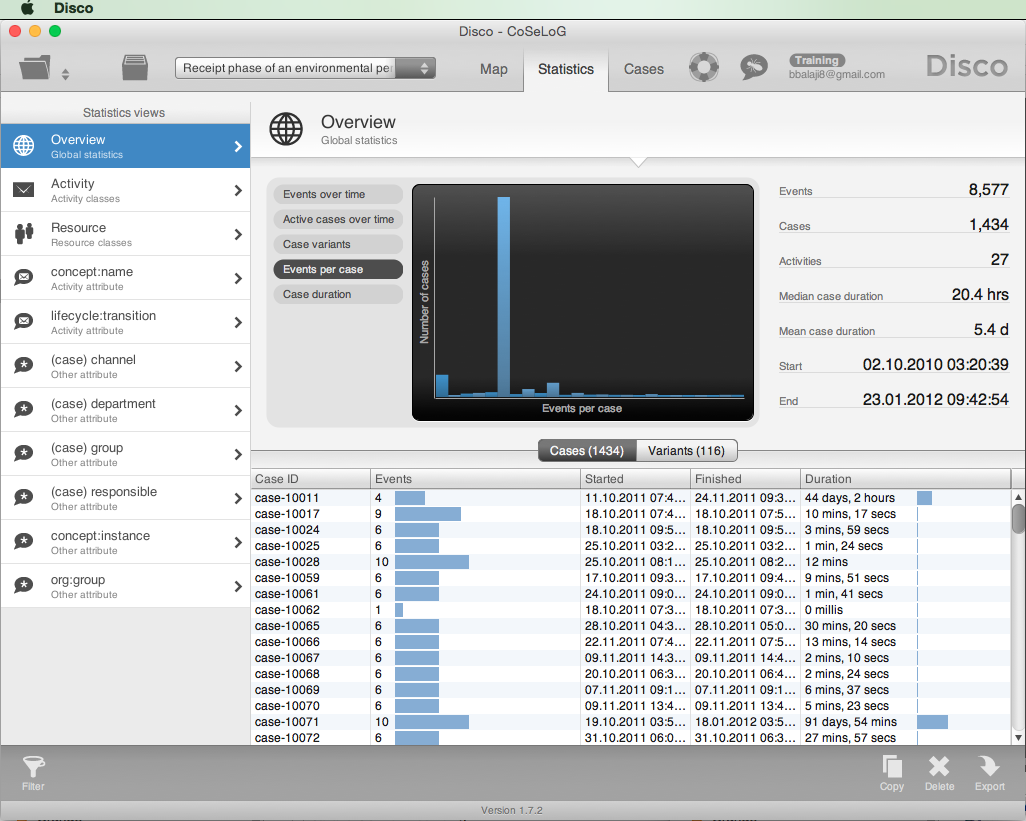
\includegraphics{CoSeLoG_Step_01_Q_01.png}

The graph pane displays a histogram (Number of cases) of Events per case
in this event log. The event log contains 8,577 events in 1,434 cases
with 27 activities.

\textbf{My analysis}:\\There are 6 events on average per case. This
information can be gathered by hovering the mouse on the tallest bar.

By clicking on ``Variants'' button on top of the table, we can see that
there are only 116 variants amongst the 1,434 cases.

The main observation from the `Events over time' graph is that the
maximum number of events (33) occured on May 2, 2011 across cases.

\subsubsection{Step 02: inspect process map in
Disco}\label{step-02-inspect-process-map-in-disco}

\textbf{Approach I used}:\\1. Click on ``Map'' tab in the window
header.\\2. Set ``Activities'' slider to 0\% \& ``Paths'' slider to 50\%
to make the process map fit on one screen and still be readable.

\textbf{What I saw}:

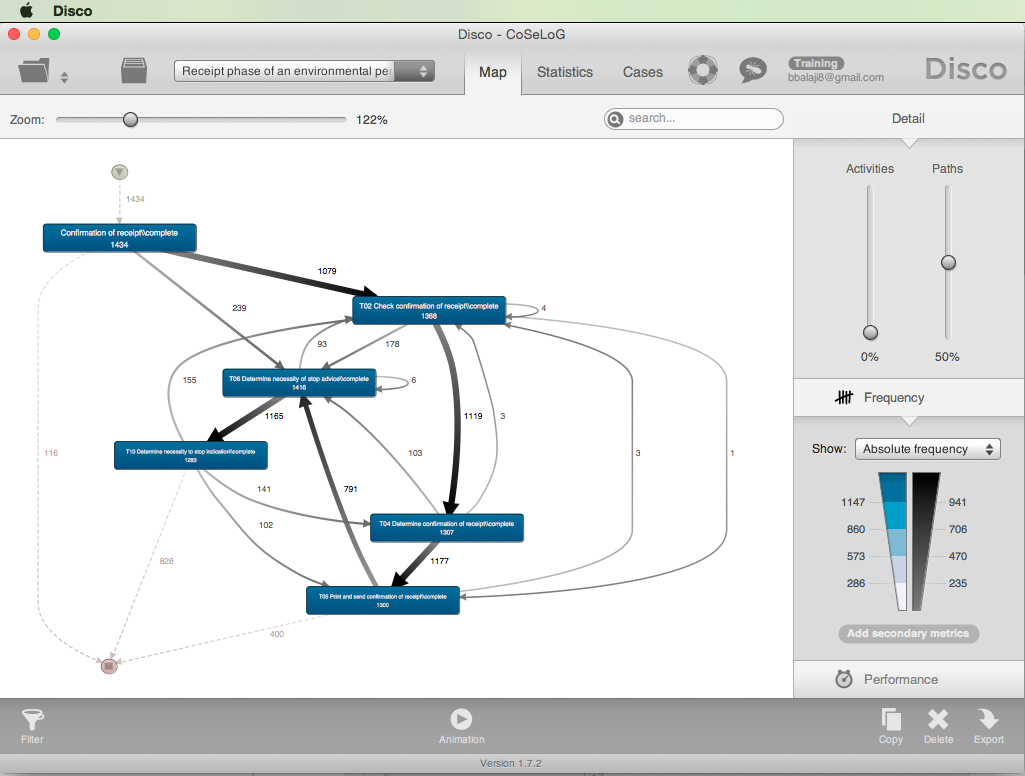
\includegraphics{CoSeLoG_Step_02.png}

\textbf{My analysis}:

The 6 most frequent activities between the initiation and termination of
cases in the process map include:\\A. Confirmation of receipt\\B. T02
Check confirmation of receipt\\C. T04 Determine confirmation of
receipt\\D. T05 Print and send confirmation of receipt\\E. T06 Determine
necessity of stop advice\\F. T10 Determine necessity to stop indication

The most frequent activity paths traced by the cases include (this is
supposed to display as a table, but doesn't work properly) :

\begin{verbatim}
                                    Activity Path | # of Cases  
\end{verbatim}

----------------------------------------------------- \textbar{}
-----------\\ Start -\textgreater{} TA -\textgreater{} End \textbar{}
116\\ Start -\textgreater{} TA -\textgreater{} T02 -\textgreater{} T04
-\textgreater{} T05 -\textgreater{} End \textbar{} 400\\Start
-\textgreater{} TA -\textgreater{} T02 -\textgreater{} T04
-\textgreater{} T05 -\textgreater{} T06 -\textgreater{} T10
-\textgreater{} End \textbar{} 828\\ \textbar{}\\ Total cases displayed
in this map \textbar{} 1,344\\ Total cases \textbar{} 1,434\\ \% cases
displayed in this map \textbar{} 94\%

Do not understand why if `` Confirmation of receipt'' is complete, there
is a need for ``T02 Check confirmation of receipt''. Additionally, there
are 4 activities (TA, T02, T04 \& T05) regarding confirmation of
receipts. Maybe these activities are not named appropriately ? and/or We
need to inspect the intermediate activities (e.g.~T01, T03) to get a
better understanding ?

\subsubsection{Step 03: inspect process performance in
Disco}\label{step-03-inspect-process-performance-in-disco}

\textbf{Approach I used}:\\1. Click on ``Performance'' bar / button in
the ``Detail'' pane (right above the ``Copy'' / ``Delete'' / ``Export''
icons).\\2. Select ``Total Duration'' in the ``Performance'' pane to
display.\\3. Select ``Case frequency'' as the secondary metric in the
``Performance'' pane to ensure that we don't use outliers (e.g.~low case
frequency) to make broad conclusions about the process.\\4. Cycle
through different metrics in the button next to ``Show:'' in the
Performance pane.

\textbf{What I saw}:

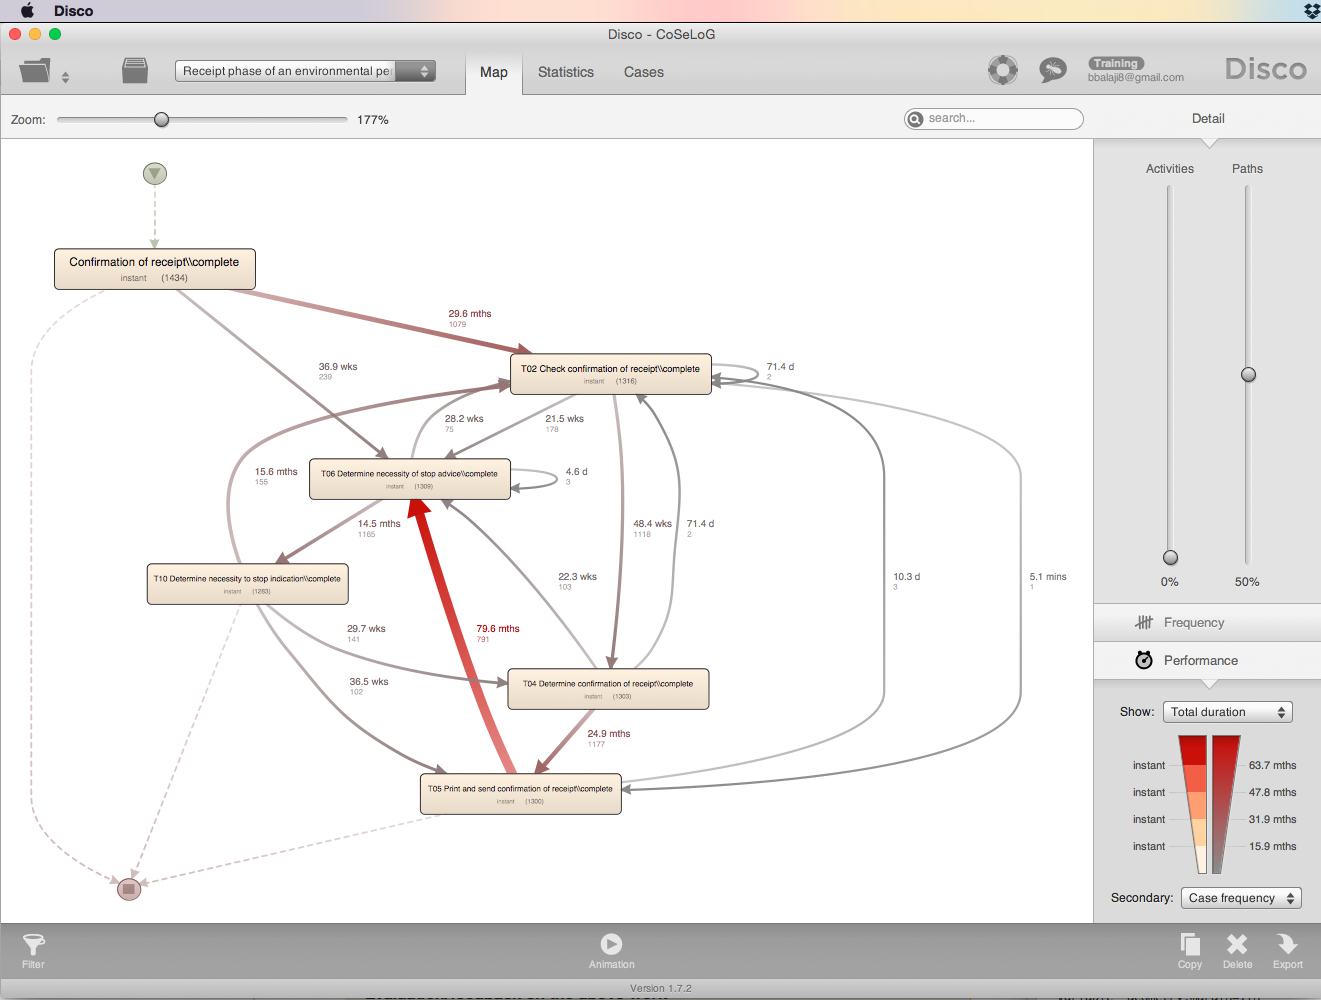
\includegraphics{CoSeLoG_Step_03.png}

The color \& thickness of the arcs are based on the distribution of the
selected primary performance metric. Additionally, if an arc is clicked,
a statistics window is dsiplayed for that arc.

\textbf{My analysis}:\\\emph{Total Duration}: The arc from T05 to T06
takes 79.6 months for 791 cases (31\% of total duration of all cases
which is 258.12 months: mean of 5.4 days per case X 1,434 cases / 30
elapsed days per month). The next bottleneck seems to be TA
-\textgreater{} T02 which is 29.6 months for 1,079 cases.

Analysis of other metrics (median, mean \& max duration) highlighted
arcs with very low case frequency.

\subsubsection{Step 04: inspect event log in
ProM}\label{step-04-inspect-event-log-in-prom}

\textbf{Approach I used}:

\begin{enumerate}
\def\labelenumi{\arabic{enumi}.}
\itemsep1pt\parskip0pt\parsep0pt
\item
  Click on ``import\ldots{}'' icon on the upper right hand side of the
  ``Workspace'' pane.\\
\item
  Click on eye icon (the one associated with the log in the middle; NOT
  the top one).\\
\item
  Click on ``Create new\ldots{}'' droplist in the top center of the
  window.\\
\item
  Select ``XDotted Chart'' by scrolling down the list.
\item
  Select ``Dotted Chart'' tab on the left.
\item
  Select ``Occurence of first event'' from the droplist for ``Case
  order:'' option.\\
\item
  Click on ``Apply Settings'' button.
\end{enumerate}

\textbf{What I saw}:

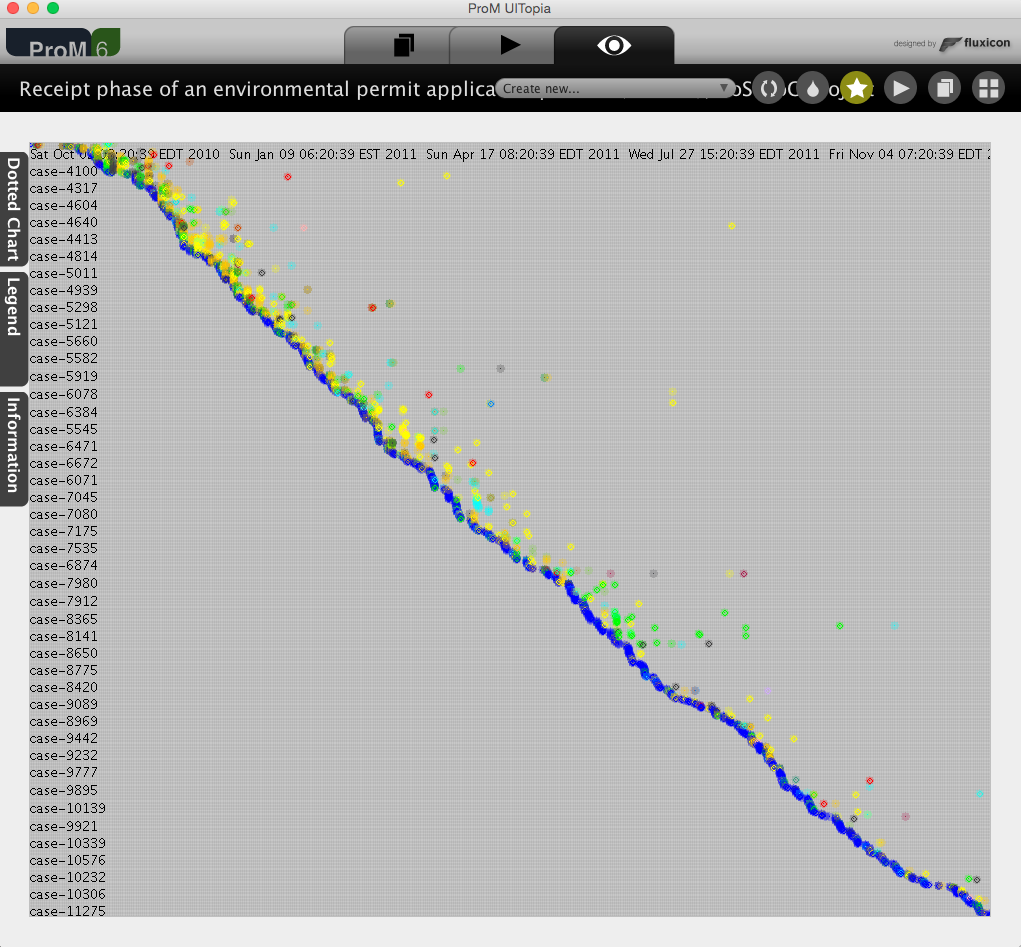
\includegraphics{CoSeLoG_Step_04.png}

Events for each case are plotted across time and color-coded. Did not
see the `size shows \# of events'-option. Zooming in does not make the
timeline any more readable / discernible (e.g.~do events initiate on
weekends ?)

\textbf{My analysis}:\\The arrival of the new cases is fairly constant
evidenced by the -45 degree slope of the (approx) line of blue dots.
There are some minor fluctuations which is difficult to quantify
(clicking on the dots does not display any additional information).

For the more recent cases there are a lot less events / activities
occuring close to case initiation compared to the earlier cases.

\subsubsection{Step 05: discover Petri net in
Disco}\label{step-05-discover-petri-net-in-disco}

\textbf{Approach I used}:

\begin{enumerate}
\def\labelenumi{\arabic{enumi}.}
\itemsep1pt\parskip0pt\parsep0pt
\item
  Click on ``Actions'' icon.\\
\item
  Add imported event log to ``Input''.\\
\item
  Search for ``Alpha'' plug-in.\\
\item
  Select ``Mine for a Petri Net using Alpha-algorithm''.
\item
  Click on ``Start'' button.
\end{enumerate}

\textbf{What I saw}:

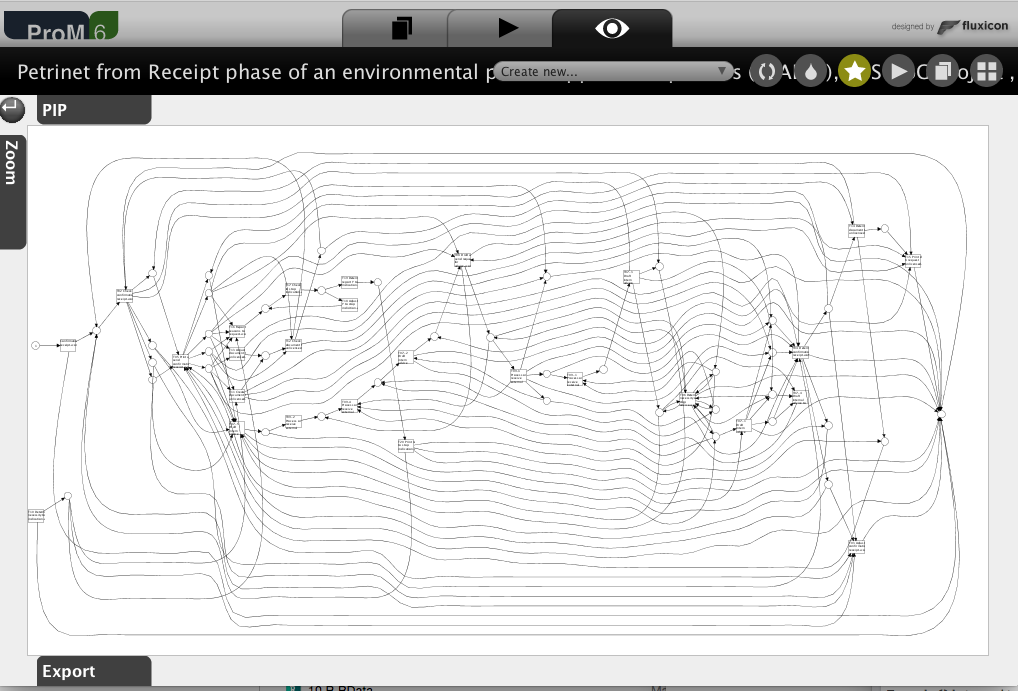
\includegraphics{CoSeLoG_Step_05.png}

This is clearly difficult to work with. Let's filter the event log to
make it more comprehensible.

\textbf{Approach I used}:

\begin{enumerate}
\def\labelenumi{\arabic{enumi}.}
\setcounter{enumi}{5}
\itemsep1pt\parskip0pt\parsep0pt
\item
  Click on ``Actions'' icon.\\
\item
  Search for ``Filter Log''.\\
\item
  Select ``Filter Log using Simple Heuristics''.\\
\item
  Click on ``Start'' button.
\item
  Change Log name to ``CoSeLoG (filtered on simple heuristics)''.\\
\item
  Click on ``Next'' button.
\item
  Select ``Select top percentage'' to 100\% because there is only 1
  Start event.
\item
  Click on ``Next'' button.
\item
  Select ``Select top percentage'' to 100\% because ideally keeping all
  End events would be critical in understanding the process.\\
\item
  Click on ``Next'' button.
\item
  Select ``Select top percentage'' to 96\% because this Event filter
  criterion discards many events and therefore many arcs in the
  resulting Petri net.
\item
  Change Log name to ``CoSeLoG (96\% filtered on simple heuristics)''.\\
\item
  Click on ``Finish'' button.
\end{enumerate}

\textbf{What I saw}:

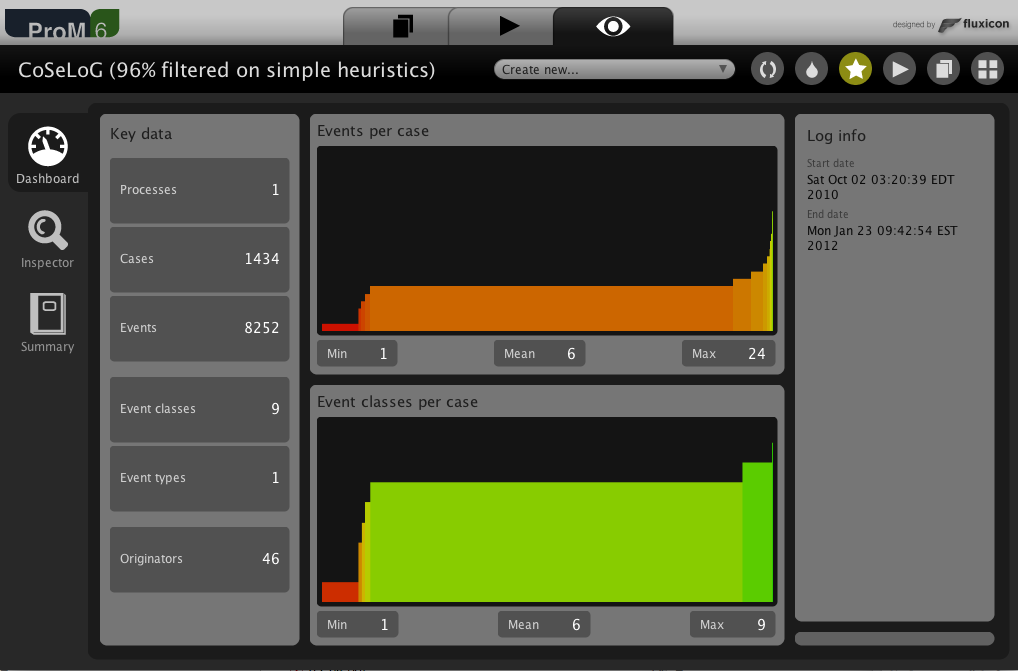
\includegraphics{CoSeLoG_Step_05_Filter96.png}

The number of Event classes has gone down from 27 to 9. The number of
Events has reduced from 8,577 to 8,252 but number of Cases remain the
same.

\textbf{Approach I used}:

\begin{enumerate}
\def\labelenumi{\arabic{enumi}.}
\setcounter{enumi}{18}
\itemsep1pt\parskip0pt\parsep0pt
\item
  Click on ``Workspace'' icon.
\item
  Select ``CoSeLoG (filtered\ldots{}''.\\
\item
  Click on ``Actions'' icon.\\
\item
  Repeat tasks numbered 1-5 listed earlier in this Step. For task 2,
  select ``CoSeLoG (96\% filtered\ldots{})'' log to ``Input''.
\end{enumerate}

\textbf{What I saw}:

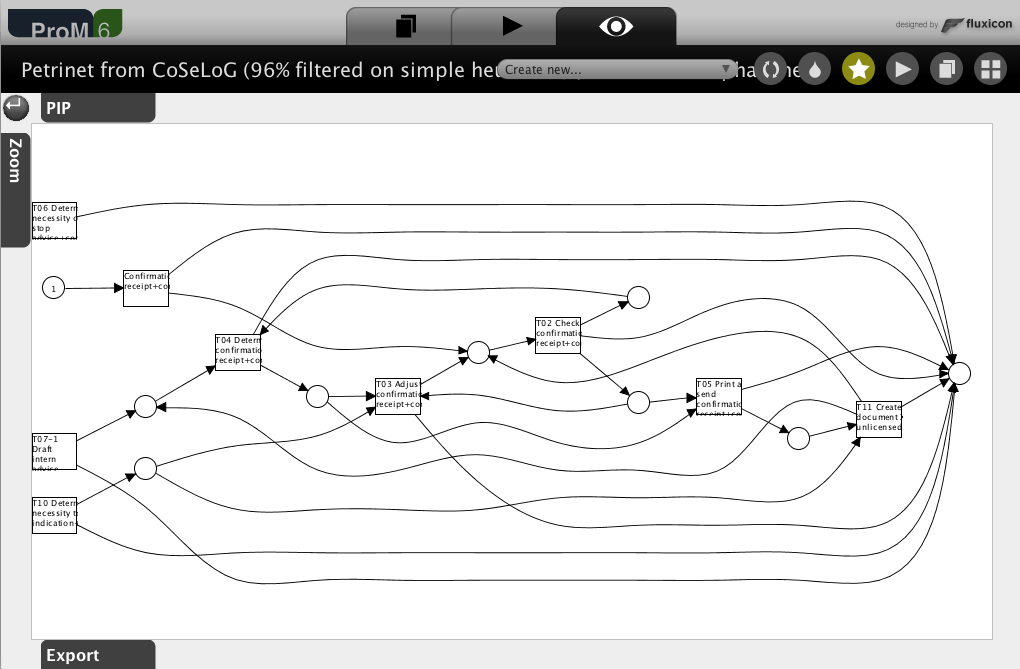
\includegraphics{CoSeLoG_Step_05_Filter96_PetriNet_Alpha.png}

The Alpha algorithm has discovered 9 transactions \& 9 places. However,
transactions T06, T07-1 \& T10 are not integrated well into the rest of
the control-flow.

\textbf{Approach I used}:

\begin{enumerate}
\def\labelenumi{\arabic{enumi}.}
\setcounter{enumi}{22}
\itemsep1pt\parskip0pt\parsep0pt
\item
  Click on ``Actions'' icon.\\
\item
  Add ``CoSeLoG (96\% filtered\ldots{})'' log to ``Input''.\\
\item
  Search for ``ILP'' plug-in.\\
\item
  Select ``Mine for a Petri Net using ILP''.
\item
  Click on ``Start'' button.
\item
  Select the ``Number of places'' option to ``Before \& After
  Transition'' instead of ``Per Causal Dependency'' to ensure clear
  ``End'' states \& minimize number of arcs.
\item
  Click ``Finish'' button.
\end{enumerate}

\textbf{What I saw}:

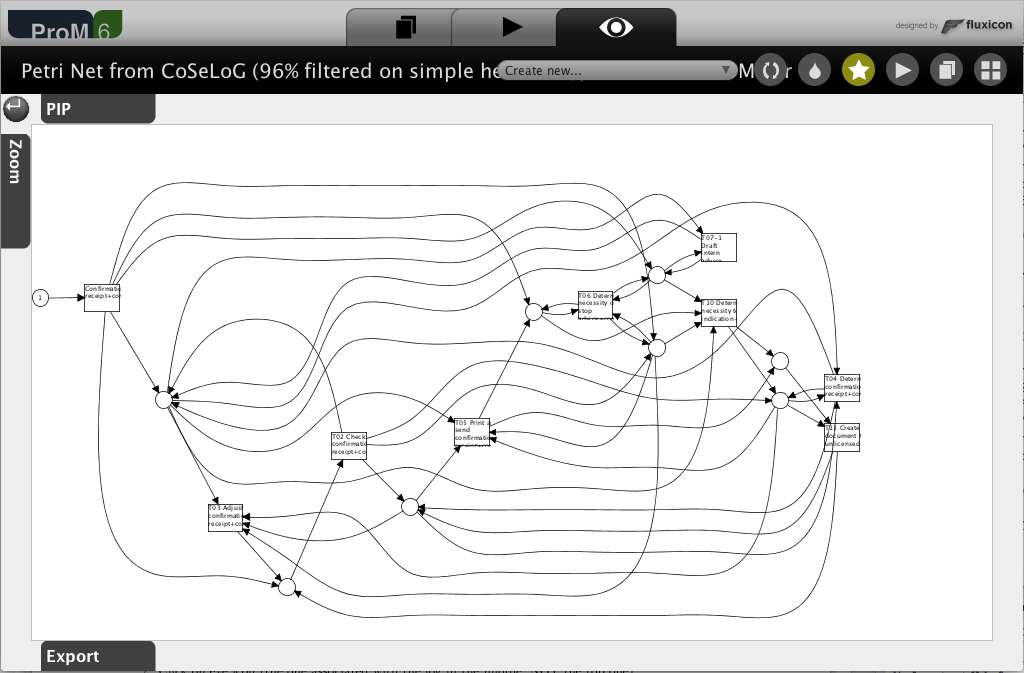
\includegraphics{CoSeLoG_Step_05_Filter96_PetriNet_ILP.png}

The ILP algorithm has discovered 9 transactions \& 8 places.
Additionally, the ILP Petri net handles transactions T06, T07-1 \& T10
better by not isolating them from the control-flow.

\textbf{Approach I used}:

\begin{enumerate}
\def\labelenumi{\arabic{enumi}.}
\setcounter{enumi}{29}
\itemsep1pt\parskip0pt\parsep0pt
\item
  Click on ``Actions'' icon.\\
\item
  Add ``CoSeLoG (96\% filtered\ldots{})'' log to ``Input''.\\
\item
  Search for ``Heuristics'' plug-in.\\
\item
  Select ``Mine for a Heuristics Net using Heuristics Miner''.
\item
  Click on ``Start'' button.
\item
  Select the default options and Click ``Continue'' button.
\item
  Click on ``Zoom'' button to the left of the graphic.\\
\item
  Select zoom level next to ``Fit \textgreater{}'' on the slider to view
  the net in its entirety.
\item
  Capture screen image.\\
\item
  Select zoom level to 50\% to make the net more readable.
\end{enumerate}

\textbf{What I saw}:

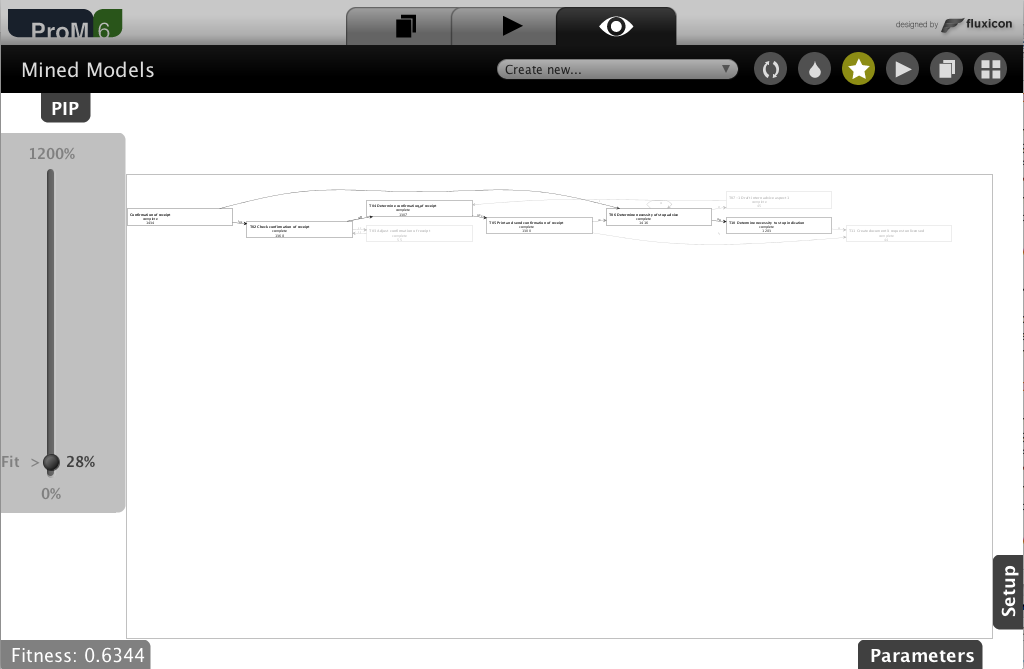
\includegraphics{CoSeLoG_Step_05_Filter96_Heuristics_Net.png}

9 transactions are discovered with a fitness score of 0.63 but T03,
T07-1 \& T11 are grayed out due to low case frequency (\textless{}= 55).

\textbf{Approach I used}:

\begin{enumerate}
\def\labelenumi{\arabic{enumi}.}
\setcounter{enumi}{39}
\itemsep1pt\parskip0pt\parsep0pt
\item
  Click on ``Workspace'' icon.\\
\item
  Select ``Mined Models'' of type ``HeuristicsNet''.\\
\item
  Click on ``Actions'' icon.\\
\item
  Select ``Convert Heuristics net into Petri net'' plug-in.\\
\item
  Click on ``Start'' button.
\end{enumerate}

\textbf{What I saw}:

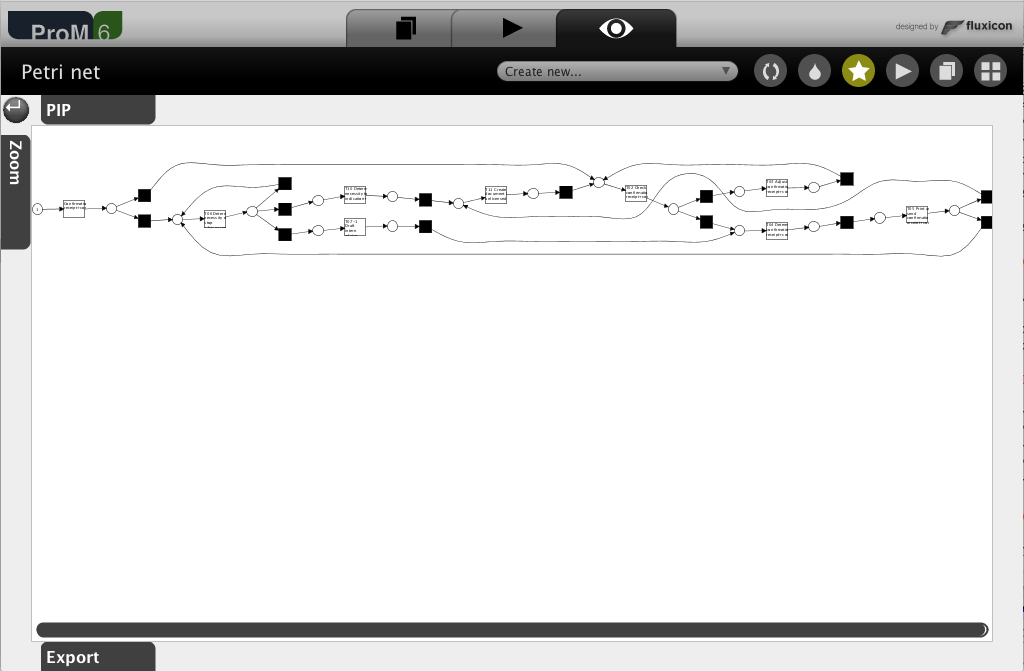
\includegraphics{CoSeLoG_Step_05_Filter96_PetriNet_Heuristics.png}

This approach has discovered 9 transactions again, 14 ``hidden'' /
``silent'' transactions and 18 places. However, there does not seem to
be a clear ``End'' place.

\textbf{Approach I used}:

\begin{enumerate}
\def\labelenumi{\arabic{enumi}.}
\setcounter{enumi}{44}
\itemsep1pt\parskip0pt\parsep0pt
\item
  Click on ``Workspace'' icon.\\
\item
  Select ``CoSeLoG (96\% filtered\ldots{})'' log.\\
\item
  Click on ``Actions'' icon.\\
\item
  Search for ``Inductive'' plug-in.\\
\item
  Select ``Mine Petri net with Inductive Miner'' plug-in.\\
\item
  Click on ``Start'' button.
\item
  Change ``Variant'' option from default of ``Inductive Miner -
  infrequent'' to ``Inductive Miner'' because the default option drops
  T04 transaction probably due to infrequent cases containing it. We
  want to keep this transaction so that we can compare the different
  Petri nets with the same set of transactions.\\
\item
  Click ``Finish'' button.
\end{enumerate}

\textbf{What I saw}:

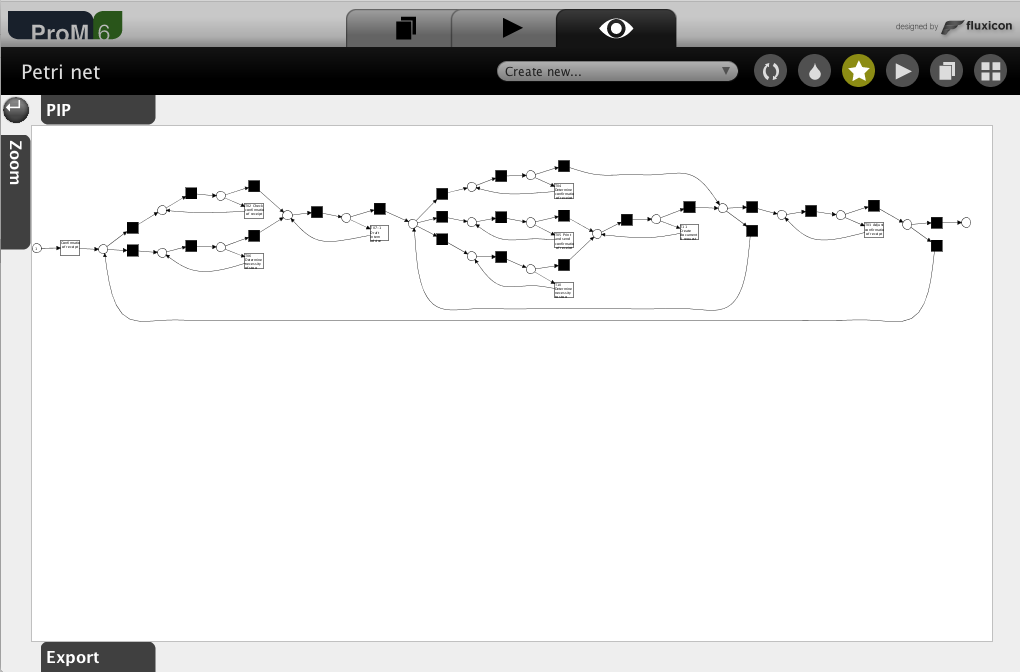
\includegraphics{CoSeLoG_Step_05_Filter96_PetriNet_Inductive.png}

This approach discovered 9 transactions, 25 ``hidden'' / ``silent''
transactions \& 21 places.

\textbf{My analysis}:

In my opinion, the ILP discovered Petri net is the best based on the
following criteria:

`+' Clear Start \& End states (ILP, Alpha \& Inductive; some combination
of options in the Heuristics plug-ins might generate a clear End state
too which I did not try due to too many steps).\\`+' Integrate all event
log transactions into the control-flow (ILP, Heuristics \&
Inductive).\\`+' No silent transactions (ILP \& Alpha).\\`+' Less arcs
(ILP \& Heuristics).

This should be displayed in a table for better readability ?

Since the analysis objective / goal is not known yet, these criteria
might be modified when that becomes clear.

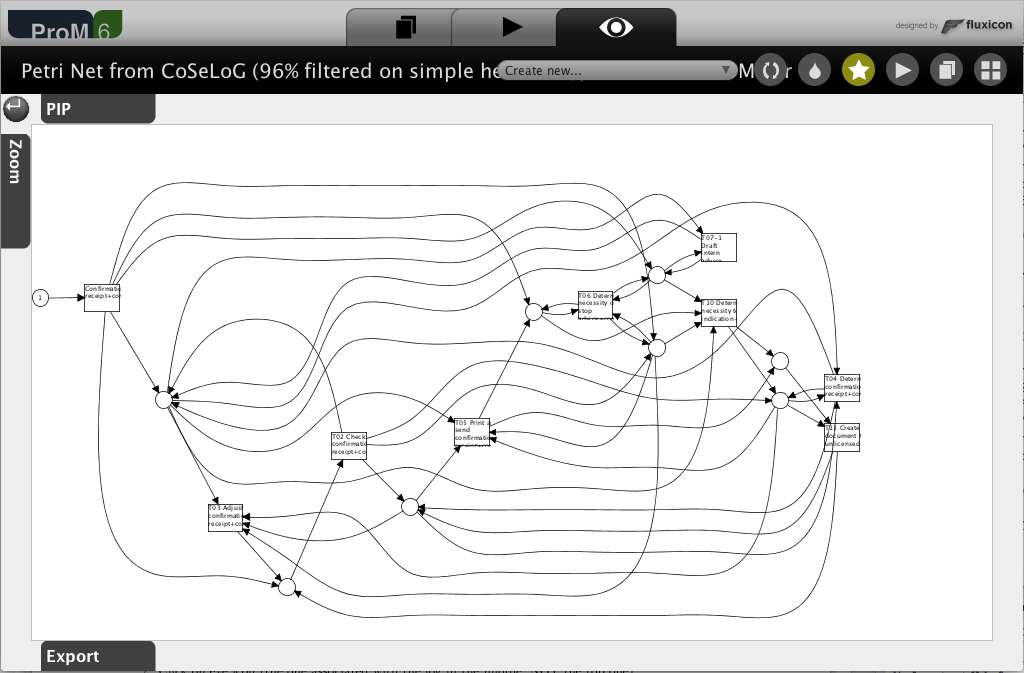
\includegraphics{CoSeLoG_Step_05_Filter96_PetriNet_ILP.png}

The main traces include:\\\textbf{1}. Start -\textgreater{} TA
-\textgreater{} T02 -\textgreater{} T05 -\textgreater{} End01 with 2
tokens remaining in ILP3 (between TA \& T10) and ILP5 (between TA \&
T07-1)

\textbf{2}. Start -\textgreater{} TA -\textgreater{} T10 -\textgreater{}
T11 -\textgreater{} End02 with 1 token remaining in ILP1 (between TA \&
T02)

The traces with some loops include:\\\textbf{1A}. Start -\textgreater{}
TA -\textgreater{} T02 -\textgreater{} {[}T04{]}* -\textgreater{} T05
-\textgreater{} End01\\ After T02, there might be any number of T04
firings

\textbf{1B}. Start -\textgreater{} TA -\textgreater{} T02
-\textgreater{} {[}T03 -\textgreater{} T02{]}* -\textgreater{} T05
-\textgreater{} End01\\ After T02, there might be any number of T03
-\textgreater{} T02 loops

\textbf{1AB}. Start -\textgreater{} TA -\textgreater{} T02
-\textgreater{} {[}T04{]}* -\textgreater{} {[}T03 -\textgreater{}
T02{]}* -\textgreater{} T05 -\textgreater{} End01\\ After T02, there
might be any number of T04 firings and/or T03 -\textgreater{} T02 loops

\textbf{2A}. Start -\textgreater{} TA -\textgreater{} {[}T06{]}*
-\textgreater{} T10 -\textgreater{} T11 -\textgreater{} End02

\textbf{2B}. Start -\textgreater{} TA -\textgreater{} {[}T07-1{]}*
-\textgreater{} T10 -\textgreater{} T11 -\textgreater{} End02

\textbf{2AB}. Start -\textgreater{} TA -\textgreater{} {[}T06{]}*
-\textgreater{} {[}T07-1{]}* -\textgreater{} T10 -\textgreater{} T11
-\textgreater{} End02

\textbf{2C1a}. Start -\textgreater{} TA -\textgreater{} T10
-\textgreater{} T02 -\textgreater{} {[}T04{]}* -\textgreater{} {[}T03
-\textgreater{} T02{]}* -\textgreater{} T05 -\textgreater{}
End01\\\textbf{2C1b}. Start -\textgreater{} TA -\textgreater{} T10
-\textgreater{} T11 -\textgreater{} T02 -\textgreater{} {[}T04{]}*
-\textgreater{} {[}T03 -\textgreater{} T02{]}* -\textgreater{} T05
-\textgreater{} End01

\textbf{2AC1a}. Start -\textgreater{} TA -\textgreater{} {[}T06{]}*
-\textgreater{} T10 -\textgreater{} T02 -\textgreater{} {[}T04{]}*
-\textgreater{} {[}T03 -\textgreater{} T02{]}* -\textgreater{} T05
-\textgreater{} End01\\\textbf{2AC1b}. Start -\textgreater{} TA
-\textgreater{} {[}T06{]}* -\textgreater{} T10 -\textgreater{} T11
-\textgreater{} T02 -\textgreater{} {[}T04{]}* -\textgreater{} {[}T03
-\textgreater{} T02{]}* -\textgreater{} T05 -\textgreater{} End01

\textbf{2BC1a}. Start -\textgreater{} TA -\textgreater{} {[}T07-1{]}*
-\textgreater{} T10 -\textgreater{} T02 -\textgreater{} {[}T04{]}*
-\textgreater{} {[}T03 -\textgreater{} T02{]}* -\textgreater{} T05
-\textgreater{} End01\\\textbf{2BC1b}. Start -\textgreater{} TA
-\textgreater{} {[}T07-1{]}* -\textgreater{} T10 -\textgreater{} T11
-\textgreater{} T02 -\textgreater{} {[}T04{]}* -\textgreater{} {[}T03
-\textgreater{} T02{]}* -\textgreater{} T05 -\textgreater{} End01

\textbf{2ABC1a}. Start -\textgreater{} TA -\textgreater{} {[}T06{]}*
-\textgreater{} {[}T07-1{]}* -\textgreater{} T10 -\textgreater{} T02
-\textgreater{} {[}T04{]}* -\textgreater{} {[}T03 -\textgreater{}
T02{]}* -\textgreater{} T05 -\textgreater{} End01\\\textbf{2ABC1b}.
Start -\textgreater{} TA -\textgreater{} {[}T06{]}* -\textgreater{}
{[}T07-1{]}* -\textgreater{} T10 -\textgreater{} T11 -\textgreater{} T02
-\textgreater{} {[}T04{]}* -\textgreater{} {[}T03 -\textgreater{}
T02{]}* -\textgreater{} T05 -\textgreater{} End01

All the traces that end in End01 have 2 tokens remaining as described
for Trace 1.\\All the traces that end in End02 have 1 token remaining as
described for Trace 2.

These traces should be in a table for better comprehension ?

\subsubsection{Step 06: inspect conformance with normative model in
ProM}\label{step-06-inspect-conformance-with-normative-model-in-prom}

\textbf{Approach I used}:

\begin{enumerate}
\def\labelenumi{\arabic{enumi}.}
\itemsep1pt\parskip0pt\parsep0pt
\item
  Click on ``Workspace'' icon.\\
\item
  Click on ``import\ldots{}'' button.\\
\item
  Select the normative model file.\\
\item
  Select the `PNML Petri net files' importer.\\
\item
  Click on ``Actions'' icon.\\
\item
  Search for ``Replay'' plug-in.\\
\item
  Select `Replay a Log on Petri Net for Conformance Analysis' (not the
  variant with performance!) plug-in.
\item
  Add original event log to ``Input''.\\
\item
  Click on ``Start'' button.\\
\item
  Click `yes' in the `No Final Marking' pop-up.
\item
  Select the `sink' place on the left (note: do not select `0-sink'
  etc.) and click the button `Add Place \textgreater{}\textgreater{}' to
  add the place `sink' to the candidate final marking list.
\item
  Click `Finish' in the mapping wizard.\\
\item
  Click `Finish' .\\
\item
  Click `No, I've mapped all necessary event classes' to indicate that
  some events are not present in the normative model.\\
\item
  Click `Next'.\\
\item
  Click `Finish'.
\end{enumerate}

\textbf{What I saw}:

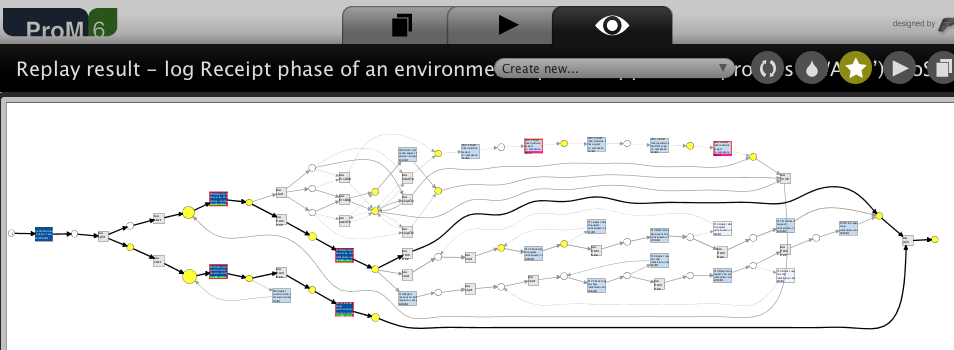
\includegraphics{CoSeLoG_Step_06_PetriNet_Normative_Conformance.png}

\emph{Transitions}: Most of the traces pass through very few ``labeled''
(tau are ``silent'') transitions: TA -\textgreater{} T06 -\textgreater{}
T10 \& TA -\textgreater{} T04 -\textgreater{} T05. The color darkness or
``fill'' of the transition boxes is based on the number of traces in the
event log that fire them. The numbers underneath the label in the
transition boxes refer to the number of synchronous moves / move on
model. T13 \& T18 are never fired in this event log.

\emph{Places}: Place size displays move on log frequency. Places where
move log occured are colored yellow. However, size of ``source'' \&
``sink'' are not adjusted. Clicking on the place displays the underlying
label. Size of places going to silent transitions are not adjusted with
frequency but are colored yellow when there are move(s) on log.

\emph{Arcs}: The thickness of the arcs seems proportional to the
frequency of event log traces.

\textbf{My analysis}:

T10 has the maximum deviations (151). T06 has the minimum (125). The
replay fitness (the `trace fitness' statistic) of the event log on the
normative process model is 0.8425.\\The transition `T06 Determine
necessity of stop advice+complete' (on the top left of the model) was
tested with 1,434 traces in the event log. Out of those 1,309 (91\%)
were synchronous moves in both the model \& log. Amongst those 1,309
traces, T06 was fired synchronously for 1,327 times (i.e.~some traces
fired T06 fired multiple times). For 125 traces, T06 was fired in the
model only.

\subsubsection{Step nn: step title}\label{step-nn-step-title}

\textbf{Approach I used}:

\textbf{What I saw}:

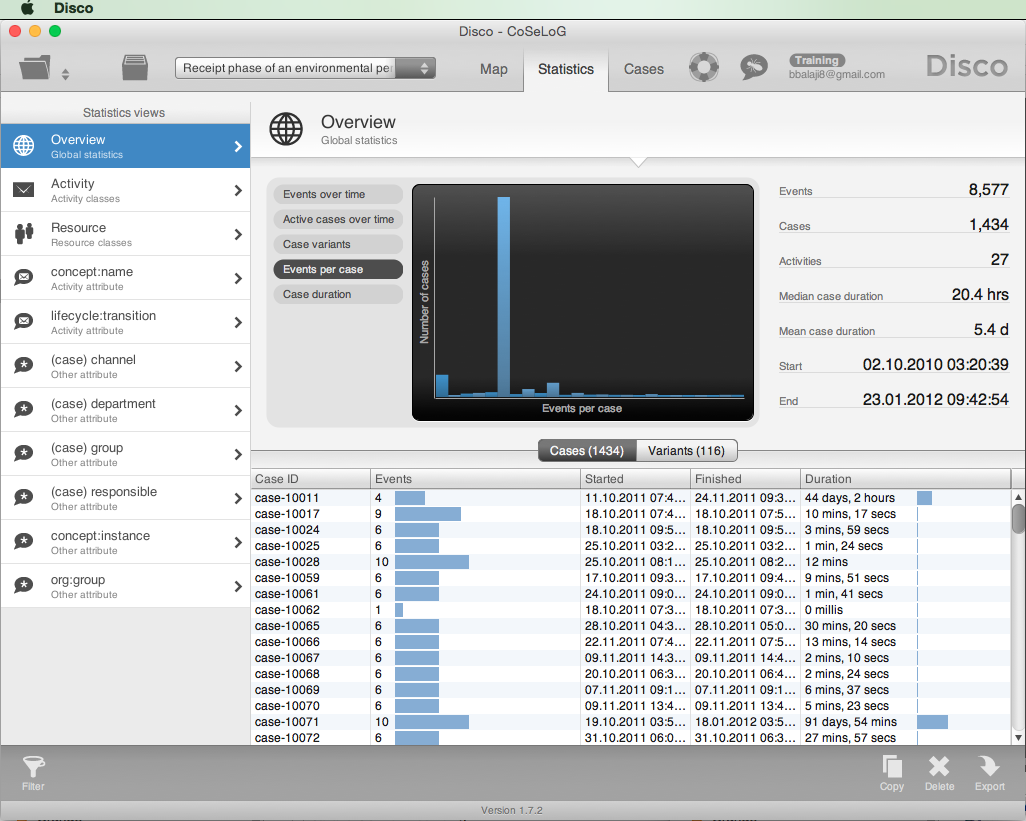
\includegraphics{dummy.png}

\textbf{My analysis}:

\end{document}
